\section{Discussion} \label{sec:discussion}

\subsection{Iterative Adjustment of the Nanosatelite Configuration} \label{subsec:disc_itt}
Iterative adjustment of the nanosatelite configuration was never implemented. We decided that we it was not possible to make a correct and non naive implementation within the given time frame of this project. We have decided to include the feature as future work as it we believe it will make the system easier to use.

The downside of having the user to manually adjust their configuration is that they have to decide on which parts of the input that have to be tuned. An automatic process could be able to analyse the schedule for bottlenecks or other parts that would be candidates for change. It can be hard o manually find the variables that may lead to schedule that is not possible, or not robust. They are also limited in what the are able to change, as it is not possible to modify all of the internal variables. Some are hidden anyway to lower the required knowledge of the internal tools, UPPAAL \gls{cora} and \gls{smc}, in order to make the system easier to use. 
%Instead of having to manually adjust the configuration, it could be possible to make the system self configurable at the end of an iteration. Either to explorer new schedules or a more aggressive robustness analysis. For example, \cref{fig:tool_act}  have added an additional step to the tool-chain by allowing the system to loop if the robustness queries were unsatisfied. The system would then have to adjust the variables, such as the [min, max]

Since the iterative adjustment of the nanosatelite configuration have become manual, we have supplied an updated version of the tool-chain which now handles a "No" and "yes" equally in location 6.
\begin{figure}[h]
	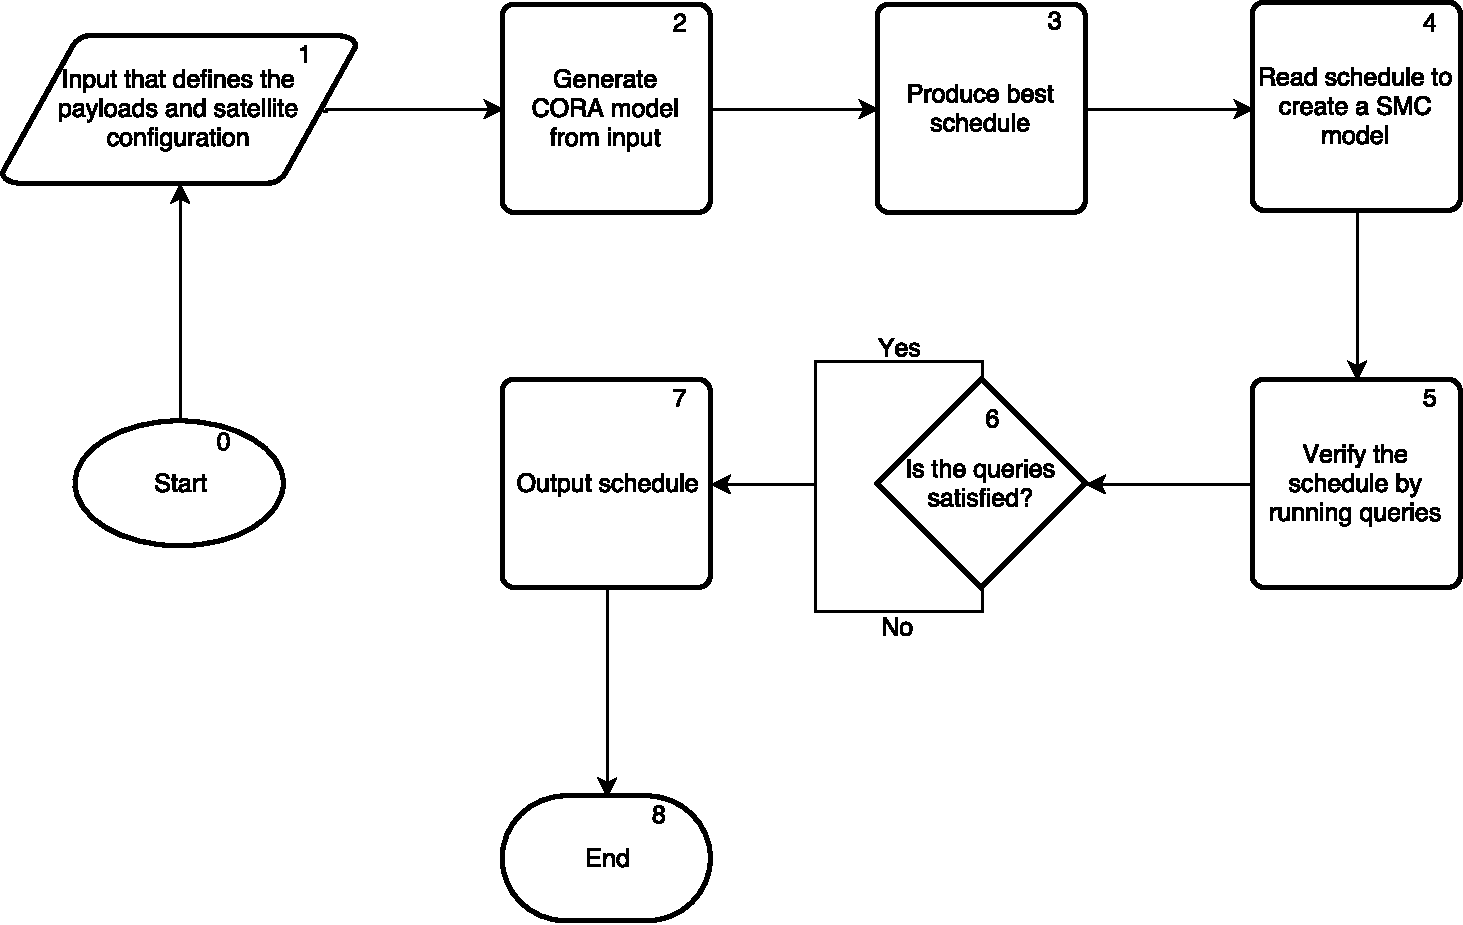
\includegraphics[width=\textwidth]{graphics/flow_act.pdf}
	\caption{Flowchart that displays the actual workflow}
	\label{fig:tool_act}
\end{figure}


\subsection{looping schedules}
problem determine SOC when a battery ends 

logic or in dependencies

\subsection{Battery Lifetime} \label{subsec:disc_life}



\subsection{Proof of viability}
Vi har kun lavet stikproever
Det tilfldige aspekt goer det besvaergeligt (Random search)

\subsection{SMC flaw}
scheduler predict cost of the next payload based on a and b? but dose not take recharge into account or the waiting period of the payload has executed, so potentially it is possible for the battery to go under the threshold if the waiting period after the payload and the next one is enough to have idle energy cost make the battery go under the threshold,  

\subsection{Improving Insolation}
As mentioned in \cref{sec:cora} the model always assume an initial state of insolation, that the nanosatellite is in the sun. Resulting in our schedule only being able to generate schedules for the nanosatellite when it matches our starting point.
This could be corrected by adding new initial location, that have transitions to both of the existing locations, given a variable that will determine which location there should be transitioned to based on the actual position of the satellite.

\subsection{Zero Windows}
As of now the models, both \gls{cora} and \gls{smc}, does not support there being no defined windows in the payload description as several variables are dependant on this. However, as windows is an important concept for our context we do not believe this to be a problem. Also there is a workaround by defining all payloads as having the window $0-OrbitTime$.
